\chapter{Conclusions and Outlook}
\label{ch:conclusion}

In our conclusion of this thesis, we present an overview on the natural extensions of our research followed by a discussion of the work completed. In Section \ref{sec:furtherwork}, we outline a particular project which has followed naturally from this thesis, whose work was started in our thermodynamic paper \cite{Gutowski:2020fzb}, and will be continued in an upcoming publication \cite{thirdpaper}. We finish the chapter with Section \ref{sec:summary} with a summary of the work undertaken in the thesis, together with some general remarks on other possible research projects. We hope that this offers a non-technical overview, helping the reader review the motivations and insights that carried us throughout this body of work.


\section{Further work}
\label{sec:furtherwork}

We begin with a result first presented in \cite{Gutowski:2020fzb} where we considered the thermodynamics of a four-dimensional planar symmetric black hole solution, derived from the so-called \emph{Einstein-anti-Maxwell} theory, which differs from the standard Einstein-Maxwell theory through flipping the sign in the gauge field coupling:
\begin{equation*}
	S = \frac{1}{16 \pi} \int d^4x \sqrt{-g} \left(-R + F^2 \right).
\end{equation*}
When compared to the cosmological solution of Chapter \ref{ch:planarem}, we find the static and dynamic regions of the solution are exchanged such that the first law and other thermodynamic relations can be derived using a conventional Wick-rotation. We will show that this planar black hole solution can be viewed as the `dual' partner to the planar cosmological solution of Einstein-Maxwell theory. This solution realises the same thermodynamical system as studied in Section \ref{sec:thermopem}, in the sense that both solutions have the same Euclidean action, and therefore the same grand potential and other thermodynamic potentials. More precisely, the range of some of thermodynamic quantities (temperature, energy) will turn out to be different, suggesting that the two solutions represent different `phases' of the same system.

In general, fields with flipped sign kinetic terms are referred to as `phantom' fields \cite{Sabra:2015vca, Taam:2015sia}. Fields with negative kinetic energy have been discussed in the context of cosmology, because some data suggest that the current expansion of the universe is over-exponential, leading to a `big-rip' cosmological singularity in finite time. While naively the negative kinetic energy renders the theory unstable, $p$-form gauge fields with inverted kinetic terms appear in the type II$^*$ string theories which are related to type II string theories by timelike T-duality transformations. In these cases, the theory is made consistent through the presence of massive string modes and the related higher gauge symmetries \cite{Hull:1998vg}. Gauge fields with flipped kinetic terms also appear in `Fake-Supergravity' theories \cite{Taam:2015sia, Townsend:2007nm}. We will return to the type II$^*$ theories shortly in the context of generalising the Einstein-anti-Maxwell theory into $\N = 2$ supergravity. 

\begin{figure}[h!]
\centering
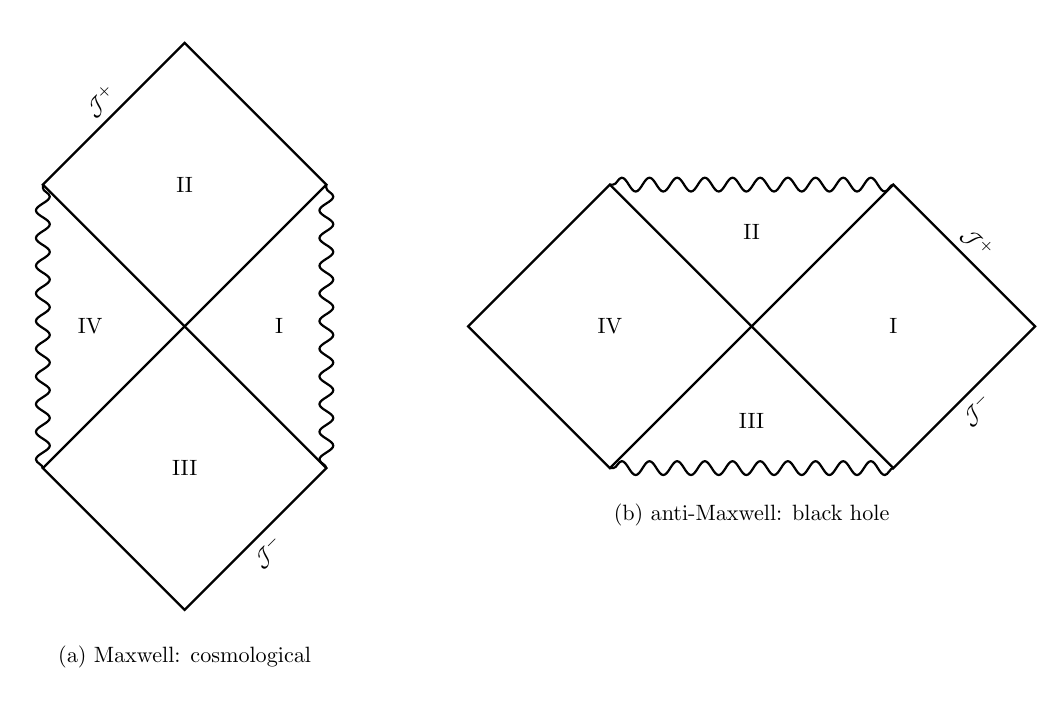
\begin{tikzpicture}[scale=0.6, every node/.style={scale=0.8}]

\node (I) at (-6,6) {II};
\node (II) at (-6,0) {III};
\node (III) at (-8,3) {IV};
\node (IV) at (-4,3) {I};
\node (label) at (-6,-4) {(a) Maxwell: cosmological};

\path % Four corners of left diamond
 (I) +(90:3) coordinate[label=90:] (IItop)
 +(-90:3) coordinate(IIbot)
 +(0:3) coordinate[label=360:] (IIright)
 +(180:3) coordinate[label=180:] (IIleft)
 ;
\draw[thick] (IIleft) -- (IItop)  node[midway, above, sloped] {$\mathcal{J}^+$} -- (IIright)  -- (IIbot) -- (IIleft) -- cycle;

\path % Four conners of the right diamond (no labels this time)
 (II) +(90:3) coordinate (Itop)
 +(-90:3) coordinate (Ibot)
 +(180:3) coordinate (Ileft)
 +(0:3) coordinate (Iright)
 ;
\draw[thick] (Ileft) -- (Itop) -- (Iright) -- (Ibot) node[midway, below, sloped] {$\mathcal{J}^-$} -- (Ileft) -- cycle;

%Squiggly lines
\draw[decorate,decoration=snake,draw=black, thick] (Ileft) -- (IIleft);

\draw[decorate,decoration=snake, draw=black, thick] (Iright) -- (IIright);

\node (Ia) at (6,5) {II};
\node (IIa) at (6,1) {III};
\node (IIIa) at (3,3) {IV};
\node (IVa) at (9,3) {I};
\node (labela) at (6,-1) {(b) anti-Maxwell: black hole};

\path % Four corners of left diamond
 (IIIa) +(90:3) coordinate[label=90:] (IIrighta)
 +(-90:3) coordinate(IIlefta)
 +(0:3) coordinate[label=360:] (IItopa)
 +(180:3) coordinate[label=180:] (IIbota)
 ;
\draw[thick] (IIlefta) -- (IItopa) -- (IIrighta) -- (IIbota) -- (IIlefta) -- cycle;

\path % Four conners of the right diamond (no labels this time)
 (IVa) +(90:3) coordinate (Irighta)
 +(-90:3) coordinate (Ilefta)
 +(180:3) coordinate (Ibota)
 +(0:3) coordinate (Itopa)
 ;
\draw[thick] (Ilefta) -- (Itopa) node[midway, below, sloped] {$\mathcal{J}^-$}  -- (Irighta) node[midway, above, sloped] {$\mathcal{J}^+$}  -- (Ibota) -- (Ilefta) -- cycle;

%Squiggly lines
\draw[decorate,decoration=snake,draw=black, thick] (Ilefta) -- (IIlefta);

\draw[decorate,decoration=snake, draw=black, thick] (Irighta) -- (IIrighta);
\end{tikzpicture}
\caption[Comparison of the Penrose-Carter diagrams of cosmological and black hole solutions.]{Comparison of the Penrose-Carter diagrams of cosmological and black hole solutions. Left side: Planar cosmological solution of Einstein-Maxwell theory. Right side: Planar black bole solution of Einstein-anti-Maxwell theory, same as for the (spherical) Schwarzschild solution of pure Einstein theory.
\label{Fig:compar}}
\end{figure}


\subsection{Planar solutions of Einstein-anti-Maxwell theory}

We start with an action which simultaneously describes both theories, 
\begin{equation*}
S = \int d^4 x \; \mathbf{e}_4 \left( - \frac{1}{2\kappa_4^2} R + \frac{\varepsilon}{4g^2} F^2\right),    
\end{equation*}
where $\varepsilon = \pm 1$ and $g^2=4\pi$ is the gauge coupling. We use vierbein notation, to avoid conflict between the spacetime metric and the gauge coupling. Introducing $g$ is convenient because it allows us to relate both theories by analytic continuation of the coupling constant $g \rightarrow ig$ leaving $\varepsilon$ fixed. Alternatively, we could relate them by analytic continuation of the gauge fields $F$, but we prefer to keep $F$ real-valued in both theories. This said, we revert to our standard conventions where $G=1, \kappa^2_4 = 8\pi$ and $g^2=4\pi$. 

Solving Einstein's equations with a static, planar symmetric ansatz yields a line element of the form:\footnote{This calculation has an almost identical discussion to the one offered in Section \ref{sec:emsolutions}, where $\varepsilon$ appears in the $R_{xx}$ component of the Ricci tensor when equated to the stress energy tensor component $T_{xx}$. Following this through, we find the charge $e^2 = Q^2$ appearing in the line element carries a factor of $\varepsilon$.}
\begin{equation}
    ds^2 = -f(r) dt^2 + f(r)^{-1} dr^2 + r^2 d\vec{X}^2,  \quad f(r) = \frac{2 C}{r} -  \frac{\varepsilon Q^2}{r^2}.
\end{equation}
As explained in \ref{sec:emsolutions}, for spherically symmetric solutions, the value of the integration constant $C$ is set by comparing the result in a weak field limit to Newtonian results. In planar symmetric theories, this is not possible as there is no asymptotically flat region. Instead, we choose the sign of $C$ by imposing the existence of a Killing horizon, which implements cosmic censorship by placing the singularity at $r=0$ behind a horizon. With this in mind, we can write the line element as
\begin{equation}
    ds^2 = -f(r) dt^2 + f(r)^{-1} dr^2 + r^2 d\vec{X}^2,  \quad f(r) = \varepsilon \left(\frac{2M}{r} -  \frac{Q^2}{r^2} \right),
\end{equation}
where the integration constant $M$ is always positive and $C = 2 \varepsilon  M$. In this form, it is easy to see that the sign of $f(r)$ is set by $\varepsilon$. Namely, when $\varepsilon = -1$, the asymptotic region is dynamic and the static patch for the solution is a finite region of the spacetime, bounded by
\begin{equation*}
0 < r < \frac{Q^2}{2 M}.
\end{equation*}
Conversely, for $\varepsilon = 1$ the static region is found for coordinate values of 
\begin{equation*}
r > \frac{Q^2}{2 M},
\end{equation*}
such that for Einstein-anti-Maxwell, the asymptotic region of the spacetime is static. Asymptotically this metric is the vacuum Taub solution \cite{Taub:1951}, with a line element
\begin{equation*}
	ds^2 = -\frac{1}{r} dt^2 + r dr^2 + r^2 (dx^2 + dy^2).
\end{equation*}
As the exterior of the solution is static, we can obtain a smooth Euclidean geometry by performing a Wick-rotation of the timelike coordinate $t$. Unlike the Einstein-Maxwell solution, here we have the standard relation between quantum mechanics and statistical mechanics, which identifies the saddle point approximation of the gravitational functional integral with a thermodynamic potential.

Setting $\varepsilon=1$, we consider the anti-Maxwell solution and calculate the Euclidean action and corresponding thermodynamic potentials. The line element in the static region is
\begin{equation}
\label{eq:planarantiem}
    ds^2 = -f(r)^2 dt^2 + \frac{dr^2}{f(r)} + r^2 d\vec{X}^2, \qquad f(r) = \frac{2M}{r} - \frac{Q^2}{r^2}, \quad r_h = \frac{Q^2}{2M}.
\end{equation}

\paragraph{Chemical potential}

The gauge field is in the same form as the solution considering in Chapter \ref{ch:planarem}, which we can write down as
\begin{equation}
    F = \left( - \frac{Q}{r} \right) dt \wedge dr, \qquad  A = \left(- \frac{Q}{r} + \frac{Q}{r_h} \right) dt,
\end{equation}
and by taking the asymptotic limit of the gauge potential, we obtain the chemical potential 
\begin{equation*}
    \mu = \lim_{r \rightarrow \infty} A_t = \frac{2M}{Q} \;.
\end{equation*}

\paragraph{Conserved charge}

The sign flip of the gauge field coupling leads to a sign flip in the conserved charge, which can be understood as relating each theory by performing $g \rightarrow -ig$ and using the Equation \eq{charges}. Therefore, the conserved electric charge is found to be 
\begin{equation*}
    \mathcal{Q} = -\frac{1}{4 \pi} \int_{\partial \Sigma} \star F = - \frac{Q}{4 \pi}.
\end{equation*}
Note that we have set $\omega=1$ for simplicity. 

\paragraph{Entropy \& Temperature}
The Einstein-anti-Maxwell solution has an exterior region with a timelike Killing vector which allows the surface gravity to be calculated by the standard method from the Killing vector field
\begin{equation*}
    \kappa = \frac{4M^3}{Q^4} \quad \Rightarrow \quad \beta = \frac{\pi Q^4}{2M^3}.
\end{equation*}
We note that using the Kodama-Hayward expression \eq{THK}, we obtain an identical result. The line element \ref{eq:planarantiem} is of the form of the \sch solution, which was discussed in Section \ref{sec:gencausalstructure}. We then realise that the horizons of the solution are outer horizons, and specifically, the horizon separating the static exterior from a dynamic interior for a future-directed causal curve is a \emph{future outer horizon}. In Figure \ref{Fig:compar} these are regions I and II in the conformal diagram on the right-hand side. This being a future outer horizon, we have $\kappa \propto T_H$ and the temperature is positive but has the same magnitude as in the Einstein-Maxwell solution.

The Bekenstein-Hawking area law gives 
\begin{equation*}
    S_{BH} = \frac{r_h^2 }{4} = \frac{Q^4 }{16 M^2}.
\end{equation*}

\paragraph{Euclidean action}
After the Wick-rotation $t \rightarrow -i \tau$ the Euclidean action is given by \eq{euclact}, with the addition of a sign flip for the gauge field contribution 
\begin{equation*}
\begin{aligned}
            S_E 
        &= \frac{1}{16 \pi} \int_M \sqrt{g} R  d^4 x  \\
        &- \frac{1}{8 \pi} \int_{\partial M} \sqrt{|\gamma|} K  d^3x + \frac{1}{8 \pi} \int_{\partial M} F^{\mu \nu} A_{\mu} d\Sigma_{\nu}.
\end{aligned}
\end{equation*}
The bulk term does not contribute, since $R=0$. 
The GHY-term is
\begin{equation*}
    -\frac{1}{8\pi} \int_{\partial M} \sqrt{\gamma} K = -\frac{3M \beta}{8\pi} .
\end{equation*} 
The gauge field contribution is identical to the one of the Einstein-Maxwell solution
\begin{equation*}
    \frac{1}{8\pi} \int_{\partial M} F^{\mu \nu}A_\mu d\Sigma_\nu = - \frac{2 M \beta}{8 \pi} ,
\end{equation*}
and when these two pieces are taken together, the Euclidean action is found to be
\begin{equation*}
    S_E = - \frac{5\beta M}{8 \pi} \;,
\end{equation*}
which is the same as for the Euclidean action of the triple Wick-rotated Einstein-Maxwell action
 \eq{emeucact}. 

As the charge is kept fixed, we associate the grand canonical thermodynamic partition function with the saddle-point approximation of the gravitational partition function:
\begin{equation*}
    \log \mathcal{Z} = -{\cal N} S_E = - \beta \Omega \quad \Rightarrow \quad \Omega(\beta, \mu) = - \frac{5 \mathcal{N} \beta \mu^4 }{(8 \pi)^2}\;,
\end{equation*}
where we have expressed $\Omega$ in terms of its natural thermodynamical variables. 
The normalisation constant $\mathcal{N}$ is fixed by imposing the relation
\begin{equation*}
    \pardev{\Omega}{\mu} = -\mathcal{Q} \;.
\end{equation*}
Since
\[
\pardev{\Omega}{\mu} = - 20 \mathcal{N}  \frac{\mu^3 \beta}{(8\pi)^2} \;,\;\;\;
- \mathcal{Q} = \frac{Q}{4\pi} = \frac{\mu^3 \beta}{(4 \pi)^2} \;, \;\;\;
\mu = \left( - \frac{(4\pi)^2 \mathcal{Q}}{\beta} \right)^{1/3},
\] 
this fixes $\mathcal{N}=-\frac{1}{5}$, so that the grand potential for the 
planar Einstein anti-Maxwell solution is
\[
\Omega(\beta, \mu) = \frac{\beta \mu^4}{(8\pi)^2} \;.
\]

The free energy is then obtained by a Legendre transformation:
\begin{equation*}
    F(\beta, \mathcal{Q}) = \Omega + \mu \mathcal{Q} =
    - 3 \left( \frac{\mathcal{Q}^4 \pi^2}{4 \beta} \right)^{\frac{1}{3}}.
\end{equation*}
By taking partial derivatives we can verify that the following two thermodynamic
relations take their standard forms:
\begin{equation*}
    \pardev{F}{\mathcal{Q}} = \left(- \frac{(4\pi)^2 \mathcal{Q}}{\beta} \right)^{\frac{1}{3}} = \mu, \qquad     S = \beta^2 \pardev{F}{\beta} = \left(\frac{\mathcal{Q}^4 \beta^2 \pi^2}{4} \right)^{\frac{1}{3}} = S_{BH}.
\end{equation*}
Therefore we are confident in defining the internal energy as
\begin{equation*}
    E = \pardev{(F \beta)}{\beta}  = -\frac{M}{4 \pi} <0 \;.
\end{equation*}
We note that $E$ is negative, which reflects that in the Einstein-anti Maxwell theory the
vector field has negative kinetic energy. 
By expressing $E$ in terms of its natural thermodynamic variables, we obtain 
the following equation of state:
\begin{equation*}
    E(S, \mathcal{Q}) = - \frac{\pi \mathcal{Q}^2}{\sqrt{S}} \;.
\end{equation*}
Finally, we compute the total differential of the internal energy, 
\begin{equation*}
    dE = \pardev{E}{S} dS + \pardev{E}{\mathcal{Q}} \mathcal{Q} = \beta^{-1} dS + \mu d\mathcal{Q},
\end{equation*}
and find that the first law is satisfied. It is interesting to note that the Euclidean action and grand potential, as well as other thermodynamic relations, are the same as for the planar solutions of Einstein-Maxwell theory, except for the range of some of the parameters. For the Einstein-Maxwell solution, the temperature is negative and internal energy is positive, while for the Einstein-anti Maxwell solution, the temperature is positive and internal energy is negative. While both solutions exhibit features indicating instabilities (negative temperature and negative internal energy, respectively), they obey all formal relations of thermodynamics and have the same underlying Euclidean action. 

The matching of partition functions for distinct theories is usually a hint towards a deeper underlying duality. In the following section, we comment on a few ideas we have been developing to study this further.

\subsection{Project outlook}

The realisation of a duality between two distinct Lorentzian solutions, via the equivalence of their Euclidean actions, has an interesting relation to recent results in ${\cal N}=2$ supersymmetry. In \cite{Gall:2019mfa}, four-dimensional ${\cal N}=2$ supersymmetry algebras have been classified for all possible signatures $(t,s)$, where $t$ is the number to timelike and $s$ the number of spacelike dimensions. A similar discussion was given for the five-dimensional case in \cite{Gall:2018ogw}. It was found that while the ${\cal N}=2$ supersymmetry algebra is unique in Euclidean signature $(0,4)$, there are two inequivalent algebras in Minkowski signature $(1,3)$, namely the standard algebra with compact $R$-symmetry group U$(2)$ and a twisted version with $R$-symmetry group U$(1,1)$. The corresponding vector multiplet theories are distinguished by relative signs between various terms in the Lagrangian, including a relative sign between Maxwell and scalar terms. Already in \cite{Sabra:2017xvx} it has been shown that a non-standard ${\cal N}=2$ supergravity theory coupled to vector multiplets with inverted signs for all Maxwell-like terms results from the dimensional reduction of five-dimensional supergravity coupled to vector multiplets with signature $(2,3)$. This theory reduces to Einstein-anti-Maxwell theory upon truncating out the matter fields and the gravitini. We remark that while vector multiplet theories in signature $(0,4)$ can likewise be obtained in two ways from five dimensions, the resulting relative signs can be removed by a suitable field redefinition, since the underlying Euclidean  supersymmetry algebra is unique up to isomorphism \cite{Gall:2019mfa}. The situation is summarised in Figure \ref{Fig:dim_red}.


\begin{figure}[!h]
\centering

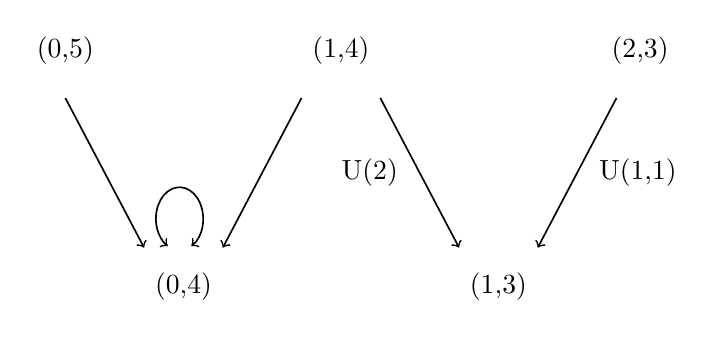
\begin{tikzpicture}[scale=2]

\node at (1,2.25) {(0,5)};
\node at (2.75,2.25) {(1,4)};
\node at (4.65,2.25) {(2,3)};

\node at (1.75,0.75) {(0,4)};
\node at (3.75,0.75) {(1,3)};

\draw[semithick,<-]  (1.5,1) -- (1,1.95) ;
\draw[semithick,->]  (2.5,1.95) -- (2,1) ;
\draw[semithick,<-]  (3.5,1) -- (3,1.95) node [midway, left=0.15cm] {U(2)};
\draw[semithick,->]  (4.5,1.95) -- (4,1) node [midway, right=0.15cm] {U(1,1)};

\draw [<->, semithick, rotate=0] (1.8,1.01) arc [start angle=-60, end angle=240, x radius=0.15cm, y radius=0.2cm];

\end{tikzpicture}

\caption[Summary of the relations between five-dimensional and four-dimensional vector multiplet theories of arbitrary signature]{This diagram summarises the relations between five-dimensional and four-dimensional vector multiplet theories with spacetime signature $(t,s)$, that is, $t$ timelike and $s$ spacelike dimensions \cite{Gall:2019mfa}. Two four-dimensional theories in a given signature differ by relative signs between terms in their Lagrangians. In Euclidean signature, these signs can be changed by a suitable field redefinition, and the Euclidean theory is unique. In Minkowski signature there are two non-isomorphic supersymmetry algebras which are distinguished by their $R$-symmetry groups U$(2)$ and U$(1,1)$, respectively. Therefore the corresponding vector multiplets theories cannot be related by a field redefinition.
\label{Fig:dim_red}}
\end{figure}


The relative sign flips between the Minkowski signature theories are of the same type as those between type II and type II$^*$ string theory, which are related to each other by timelike T-duality \cite{Hull:1998vg}. By performing a series of timelike and spacelike T-dualities, one can map between four II string theories:
\begin{equation*}
	\text{IIA} \underset{S_T}{\longleftrightarrow} \text{IIB}^* \underset{S_R}{\longleftrightarrow} \text{IIA}^* \underset{S_T}{\longleftrightarrow} \text{IIB} \underset{S_R}{\longleftrightarrow} \text{IIA}.
\end{equation*}
where we denote a spacelike (timelike) T-duality by $S_R$ ($S_T$). Moreover, $\N = 2$ supergravity with vector (and hyper) multiplets arises by compactification of type II string theory on Calabi-Yau threefolds. In a future publication, we will present the details of the embedding of the twisted $\N=2$ supergravity theory into type II$^*$ theory, where we find that beginning with one of the four type II theories, we obtain four $\N = 2$ Lagrangians when reducing over the \textit{same} Calabi-Yau manifold:
\begin{equation*}
\begin{aligned}
	&\text{IIA} \quad &&\longrightarrow \qquad \N = 2 \; (N, M) \\
	&\text{IIB} \quad &&\longrightarrow \qquad \N = 2 \; (M, N) \\
	&\text{IIA}^* \quad &&\longrightarrow \qquad \N = 2 \text{ twisted } (N, M) \\
	&\text{IIB}^* \quad &&\longrightarrow \qquad \N = 2 \text{ twisted } (M, N)
\end{aligned}
\end{equation*}
Where $(N,M) = (n_V, n_H)$ count the number of vector/hyper multiplets respectively. The values of $N,M$ are set by the specific choice of the Calabi-Yau. Finally, once in four dimensions, we turn to the c-map. Performing a spacelike c-map and then uplifting back to four dimensions, one obtains the well-known result of being able to interchange the number of vector and hyper multiplets. This is equivalent to reducing either IIA or IIB string theory over the same Calabi-Yau manifold. We extend this discussion, showing that by performing successive timelike and spacelike c-maps, one can move between all four (twisted) $\N = 2$ supergravity theories. A summary of these mappings are presented as a cube in Figure \ref{fig:cube}.

\begin{figure}[!h]
	\centering
	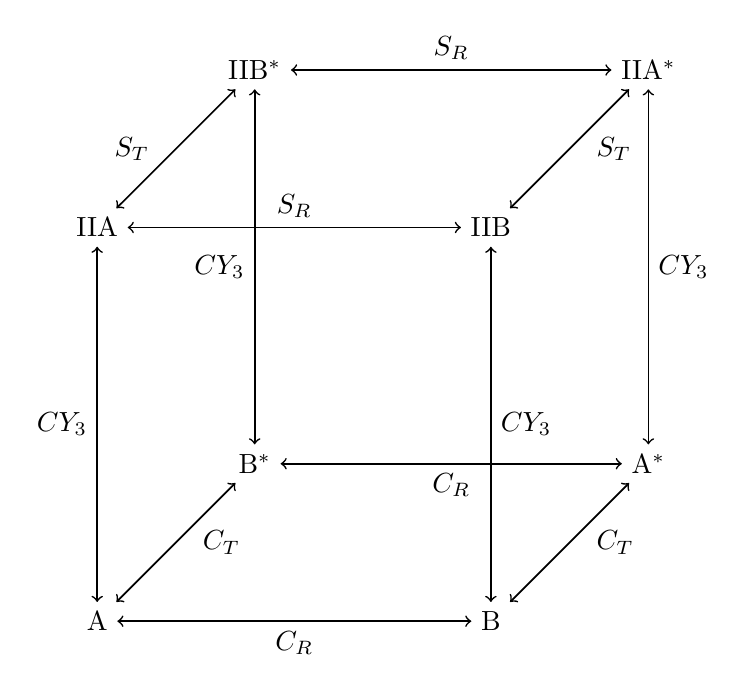
\begin{tikzpicture}	
%		base
		\node (00) at (0,0) {A};
		\node (01) at (7,2) {A$^*$};
		\node (02) at (2,2) {B$^*$};
		\node (03) at (5,0) {B};
		\draw[semithick,<->] (00) -- (03) node [midway, below] {$C_R$};
		\draw[semithick,<->] (01) -- (02) node [midway, below] {$C_R$};
		\draw[semithick,<->] (01) -- (03) node [midway, right] {\; $C_T$};
		\draw[semithick,<->] (00) -- (02) node [midway, right] {\; $C_T$};
%		top
		\node (10) at (0,5) {IIA};
		\node (11) at (7,7) {IIA$^*$};
		\node (12) at (2,7) {IIB$^*$};
		\node (13) at (5,5) {IIB};
		\draw[semithick,<->] (10) -- (13) node [midway, above] {$S_R$};
		\draw[semithick,<->] (11) -- (12) node [midway, above] {$S_R$};
		\draw[semithick,<->] (11) -- (13) node [midway, right] {\; $S_T$};
		\draw[semithick,<->] (10) -- (12) node [midway, left] {$S_T$ \;};
%		legs
		\draw[semithick,<->] (00) -- (10) node [midway, left] {$CY_3$};
		\draw[semithick,<->] (01) -- (11) node [midway, right] {$CY_3$};
		\draw[semithick,<->] (02) -- (12) node [midway, left] {\; $CY_3$};
		\draw[semithick,<->] (03) -- (13) node [midway, right] {$CY_3$ \;};
	\end{tikzpicture}
	\caption[Cube of mappings of various theories in ten and four dimensions]{On the base of the cube, we have 4 different $\N = 2$ theories. Spacelike and timelike c-maps are denoted by $C_R$, $C_T$. Theories $A$ and $B$ have $(n_V, n_H) = (N,M), (M, N)$ respectively. The theories $A^*, \; B^*$ have the same structure, but they have a non-compact $R$-symmetry. The twisted theories have Lagrangians with positive-definite gauge couplings. The top of the cube is the T-duality mapping between the type II and type II$^*$ theories. The top and base of the cube are mapped to each other by dimensional reduction over a Calabi-Yau threefold. }
	\label{fig:cube}
\end{figure}

The research then continues looking at planar symmetric solutions of the twisted supergravity theories and we find a solution to the so-called \emph{anti-STU model} which is a theory of twisted $\N = 2$ supergravity coupled to three vector multiplets where the gauge coupling has a flipped sign. We show that in much the same way we can recover the Einstein-Maxwell theory from the STU model, one can recover the Einstein-anti-Maxwell theory from the anti-STU model. We expect that continuing this research will shed more light onto the thermodynamics of planar solutions and their microscopic interpretation in terms of string theory. We remark that when combining timelike and spacelike T-duality with S-duality, it is possible to change spacetime signature in type II string theory, which provides a second way besides analytical continuation, of relating theories in Euclidean and in Minkowski signature \cite{Hull:1998ym}. Solutions in neutral and in general signature have recently found attention in the literature, see for example \cite{Klemm:2015mga, Gutowski:2019hnl, Sabra:2020gio}.

However, we must be careful with the distinction between the symmetry between Lagrangians and that of solutions. From a string-theory perspective, we can relate Lagrangians with flipped signs through performing a timelike, then spacelike T-duality. From the four-dimensional perspective, we can map theories to one another by performing consecutive spacelike and timelike c-maps. However, when we solve the equations of motion for these planar symmetric theories, there is an additional restriction made to ensure the presence of the Killing horizon. For the (anti)-Einstein-Maxwell solutions, we saw this as the setting of the sign of $C$. For the STU model in \ref{sec:4dSolutions}, this was achieved through a set of regularisation conditions. Neither of these restrictions can be captured by the above duality transformations, but rather must come from some other perspective.

Let us take the simpler solutions of the (anti)-Einstein-Maxwell solutions. If we imagine that the sign of $C$ is fixed and we perform a duality transformation, we would expect to have a mapping between a solution containing a Killing horizon to a solution containing a naked singularity (and vice-versa). We would only expect to map Killing horizons into each other if we also flipped the sign of $C$ (which we could equally well understand from flipping the sign of the mass $M$). This behaviour is expected from another perspective from the history of literature of black holes and T-duality transformations (usually studied in the low-energy limit with the Buscher rules). Although the Killing horizon is preserved for spacelike symmetries \cite{Horowitz:1993wt}, this is not the case of timelike dualities \cite{Rocek:1991ps}. Further discussion on this is given in \cite{Arvanitakis:2016zes}, where the authors comment on the mapping between naked singularities and black hole solutions while formulating a manifestly T-dual invariant discussion of the first law of thermodynamics. The duality between naked singularities and black holes is also discussed in \cite{Rinaldi:2002tc, Manko:2018yrc}. Another instance of mapping between solutions with horizons and naked singularities is discussed in \cite{Dijkgraaf:2016lym} when studying negative brane solutions in string theory.\footnote{We became aware of this paper when first studying these cosmological solutions in \cite{Gutowski:2019iyo}, when the negative-definite mass-parameter of the four-dimensional solution in the static patch seemed to hint that our solutions were negative branes, although this was not followed up after we worked with the extremal limit and studied our solutions as intersecting brane solutions.}

One idea we wish to follow in more detail is considering planar solutions to each theory not as four distinct solutions where $C$ is constant, but rather as pairs of theories with $C$ permitting both signs: one with a Killing horizon and one with a naked singularity. The conjecture we make is that flipping the sign of $C$ maps solutions within a theory between spacetimes containing a Killing horizon or a naked singularity and that T-duality maps solutions with or without a Killing horizon between theories. We also notice that `flipping the sign' of $C$ could also be understood as the continuation through the singularity. This would allow $C$ to remain fixed, and for the Killing horizon to appear (disappear) by considering $r < 0$. This continuation to glue together regions at singularities has been considered for the \sch solution \cite{Araya:2015fva} where the authors consider the different interpretations of flipping the sign of the gravitational coupling, or continuations through the singularity.

Both from the point of view of thermodynamics and from the one of T-duality, certain spacetime geometries naturally form pairs which share the same underlying Euclidean description. If one takes the Euclidean functional integral as fundamental and allows both the spacetime and the field space to be complex-valued, this will correspond to pairs of complex saddle points of the functional integral which represent dual Minkowksi signature solutions. At this point it is not clear whether the two dual solutions are actually `the same', that is, gauge equivalent under a chain of string duality transformations, or just have `the same thermodynamics.' In either case, one could also look for relations to solutions in neutral signature. It will be interesting to further investigate these intriguing relations between geometry, thermodynamics and dualities. 

\section{Summary}
\label{sec:summary}

In this thesis, we have presented a discussion on four-dimensional planar symmetric solutions and their thermodynamics. Using the c-map and the real formulation of special geometry, we derived a class of non-extremal cosmological solutions of $\N = 2$ supergravity containing a Killing horizon. Our analysis of the extremal limit of these solutions led to the discussion of our four-dimensional solutions embedded into string/M-theory and the recovery of supersymmetric solutions in six dimensions. Validating the first law of thermodynamics led to the development of a novel formulation of the Euclidean action formalism. In this chapter, we briefly discussed future work inspired by the implied duality found from the matching of Euclidean partition functions for distinct theories related by the flipping of the sign for the gauge coupling in the Lagrangians. 

Our discussion began considering planar symmetric solutions of Einstein-Maxwell theory in Chapter \ref{ch:planarem}. Following the example of the Reissner-Nordstr\"om solution (Section \ref{sec:rnsol}), we derived the line element by solving Einstein's equations, imposing that the spacetime was planar symmetric and static. To ensure the presence of a Killing horizon, we set the sign of the integration constant: $C = -2M < 0$, and noticed that for $C \geq 0$ the solution contained a naked singularity, violating the cosmic censorship conjecture. Studying the global structure of the planar symmetric solution, we found that the transverse coordinate $r$ had finite extension from the horizon at $r = r_h$ to the timelike curvature singularity at $r = 0$. We understood this static patch of spacetime in analogy to the region behind the Cauchy horizon for the Reissner-Nordstr\"om solution. Extending the geometry of the solution by introducing Eddington-Finkelstein coordinates, we then analytically continued through the horizon into a new region of the spacetime in which our transverse coordinate $r$ became timelike, and the coordinate $t$ became spacelike. For $r > r_h$, the spacetime depended only on a timelike coordinate and taking the limit of $r \rightarrow \infty$, the asymptotic geometry was understood to be that Kasner type-D vacuum solution. This time-dependent exterior geometry is what led to the naming of these \emph{cosmological} solutions. Computing the surface gravity, we identified $M \to 0$ as the extremal limit of the solution. Applying this limit, we found that the horizon was `pushed out' to infinity; the dynamic patch of the region shrank to zero size, and the resulting spacetime was everywhere static, with a naked singularity.

We then considered the static patch and studied the geodesics and conserved charges of the solution. It was found that all causal geodesics were repelled by the singularity, with the exception of the null, transverse geodesics which necessarily would reach the singularity in finite affine parameter. We understood this by interpreting the geodesic equation as the equation of motion of a massive particle coupled to a positive (repulsive) potential. Studying the trajectories, the potential ensured the existence of a classical turning point for timelike and non-transverse null geodesics. As a result, these geodesics would never reach the singularity, but would instead be repelled and continue through a Killing horizon. For null, transverse geodesics, the effective potential was zero and hence the geodesic experiences no repulsion. An alternative point of view was then offered, studying the proper acceleration for a static, massive observer. We found that the acceleration for a massive particle following orbits of the timelike Killing vector field was negative, indicating the experience of a repulsive force. Using Gauss' law, we computed the conserved electric charge (density) of the solutions, and we offered a discussion on computing a mass-like parameter for the solution. As the solution was not asymptotically flat, and the asymptotic region not stationary, we considered position-dependent mass-like quantities within the static region using both the Komar energy and quasi-local energies. However, we found no natural normalisation for our calculations, and so we could at most comment on the overall sign, which we found was everywhere negative for all treatments. We also noted that for the Komar energy and the Katz-Lynden-Bell-Israel quasi-local energy, we could take the asymptotic limit and find a finite quantity. Usually taking this limit for the Komar energy is associated with the Komar mass under the assumption that the solution is asymptotically flat and stationary. As the planar symmetric solution had neither of these properties, we could not draw the same conclusion. Instead, as asymptotically the conserved charge is computed from a spacelike isometry, the finite quantity could be thought of as a conserved momentum, generated by translations at asymptotic infinity. Later in the thesis, this conserved charge would appear again as the internal energy of the solution from a thermodynamic perspective.

We concluded our discussion considering the global structure of cosmological solutions, allowing the line element to be generalised to not only cover the planar solutions of Einstein-Maxwell theory but also for the planar solutions of the STU model and the de Sitter solution when written in static coordinates. In this general form, we were able to write down the Kruskal coordinates for the solutions and from them, the corresponding Penrose-Carter diagrams. Following a discussion first offered in \cite{Gutowski:2020fzb}, we then carefully studied each of the four regions and showed that following our conventions, the spacetime region IV could be understood as having the conventional flow of time (see Figure \ref{fig:sub2}). Using the expansions of null geodesic congruences, we were then able to classify the horizons. We found that the horizon between regions III and IV was a \emph{future inner} horizon and the horizon between regions II and IV was a \emph{past inner} horizon (see Figure \ref{fig:flipped}). The classification of the horizons allowed us to set the sign of the temperature from the Kodama-Hayward surface gravity, which we would need when applying the Euclidean action formalism. To match the standard case for the \sch solution, we would consider the future inner horizon, which is crossed by future-directed, causal geodesics travelling from the external to the internal regions of the solution. For future inner horizons, the Hawking temperature is proportional to the surface gravity, which is negative for the solutions we discussed within this section.  

We then turned to study the planar symmetric solutions of the STU model. This research was the initial starting point for the work presented in this thesis, and the previous discussion of the solutions of Einstein-Maxwell theory serves as the minimal example, which can be recovered from the STU model through the restriction that the scalar fields are constant throughout the spacetime. This relationship between the more complex solutions of $\N = 2$ supergravity coupled to vector multiplets and the familiar Einstein-Maxwell theory allowed us to build upon already established ideas, helping to give space for the more involved discussions particular to the solution generating method employed within this chapter.  

Our work was motivated through wanting to consistently generalise the Nernst brane solutions of \cite{Dempster:2015}. The Nernst branes are non-extremal solutions of $\N = 2$ gauged supergravity coupled to an arbitrary number of vector multiplets with a single electric charge. Their defining characteristic was that in the extremal limit, the area (density) of the Killing horizon vanished and so could be understood as black hole solutions obeying the strict third law of thermodynamics. Our goal was to look at increasing the number of charges, and in \cite{Gutowski:2019iyo}, we presented a discussion of dyonic solutions with one electric charge and between one and three magnetic charges. With the interesting thermodynamic properties of the Nernst brane, it is natural to then to think about the thermodynamics of the multi-charged solutions. Analysing the three multi-charges solutions, we found that the solutions no-longer obeyed the Nernst law. However, for the three and four charged solutions, we instead had the surprise of deriving cosmological solutions, despite having imposed staticity while solving the equations of motion. In this thesis, we focused on the four charge solution which was a solution of the well known STU model, and this static ansatz producing a cosmological solution could be understood in analogy to the Einstein-Maxwell solution of the previous chapter.

To obtain the four-dimensional solutions, we built upon a growing history of work which employs the c-map to derive non-extremal solutions to $\N = 2$ supergravity. Starting with the STU model, the solution is assumed to be static, and subsequently dimensionally reduced over a timelike circle to produce a three-dimensional Euclidean theory. In three dimensions, the Hodge-star operator dualises vectors into scalars, and we can consistently write the three-dimensional field content as $2n_V + 2 = 8$ real scalar fields. The real formulation of special geometry allows us to write our theory in a symplectically covariant way, and the integration of the equations of motion can be done exactly after making suitable restrictions on the field content. For our solutions, this was achieved by making the purely imaginary field content restriction, and through integration of the field equations, we wrote down a Euclidean instanton solution in three dimensions. Using previously established relations, we could then uplift the solution back into four dimensions, where the resulting spacetime is necessarily static. Additionally, for our discussion, planar symmetry was imposed for the three-dimensional solution; however, this procedure would work equally well for spherical symmetry and could also be extended to consider hyperbolic symmetry.

The four-dimensional solutions were then regularised by ensuring that the presence of a Killing horizon with finite area density and that the physical scalar fields when evaluated on the horizon were not divergent. Regularisation placed restrictions on the integration constants of the theory, and we noted that this reduction of the number of remaining integration constants had similar behaviour as the restrictions from considering the attractor mechanism for non-extremal solutions. We noted that this would be an interesting avenue for further work through its possible relation to the contemporary work of the hot-attractors \cite{Goldstein:2014gta, Goldstein:2018mwt} . Given the four-dimensional solution, we then studied the null geodesics of the spacetime and identified the asymptotic geometry by identifying the region for which a null geodesic would take infinite affine parameter to reach. Using curvature scalars, we found the location of four curvature singularities. However, as we must terminate the transverse coordinate at physical singularities in our manifold, we only considered the location of the first one, which could be picked without loss of generality through ordering the magnitudes of the integration constants. We noticed that the canonical coordinates used for these solutions were not appropriate, and by making a change of coordinates, it became apparent that the transverse coordinate had finite extension within the static region between the Killing horizon and the curvature singularity. Analytic continuation through the horizon produces a new region of the spacetime which is dynamic, and we understood the planar symmetric solution of the STU model as cosmological, in direct analogy to our previous analysis of the planar symmetric solutions of Einstein-Maxwell.

Following from this similarity, we then showed explicitly that the global structure of these solutions were identical to the planar symmetric solutions of Einstein-Maxwell theory. Asymptotically, the spacetime geometry was that of the Kasner type-D vacuum solution, and taking the extremal limit had the same effect of `pushing out' the horizon to infinity, leaving behind a static spacetime containing a naked singularity with the area density of the horizon diverging. From the generalised discussion from the previous chapter, we knew that the horizons would be inner horizons and that the horizon crossed by future-directed causal geodesics passing from the exterior to the interior would cross a future inner horizon. Again, this would be important for the later thermodynamics, where the Hawking temperature was proportional to the Kodama-Hayward surface gravity which we found was negative. We studied the geodesic motion within the static region and found that the singularity was repulsive using identical considerations as from the previous chapter. We showed explicitly that for all geodesics (with the exception of null, transverse ones) there existed a classical turning point and hence geodesics could never reach the singularity. This was signalled both by the positive effective potential appearing in the geodesic equations and the negative proper acceleration for static, massive particles. The mass-like parameter has the same story as the Einstein-Maxwell discussion, where only a position-dependent quantity can be sensibly computed from either the Komar or quasi-local formalisms. Without extra information to set a normalisation, we could only conclude that the energy was negative-definite within the static region. Allowing ourselves to play with certain parameters, we again found a constant, conserved quantity associated to taking the asymptotic limit for the Komar energy and the Katz-Lynden-Bell-Israel energy. These quantities, like in the planar solution of Einstein-Maxwell, would appear again when computing the thermodynamic internal energy.

We concluded the chapter by looking at the steps needed to restrain the integration constants such that the Einstein-Maxwell theory was recovered from the STU model. We found that by ensuring all the harmonic functions $\Ham_a$ were equal, the scalar fields of the theory were constant throughout the spacetime and the resulting solution could be mapped to the solutions of the previous chapter. We noticed that applying this coordinate transformation gave us a way to express the parameter $M$ of the Einstein-Maxwell solution to the integration constants $\alpha, \gamma$ of the simplified solution of the STU model. 

The development of the cosmological solutions of the STU model from the Nersnt solutions immediately offered interesting questions. For the four-dimensional solutions of \cite{Dempster:2015}, there were divergences of the scalar fields in the asymptotic limit and infinite tidal forces as one approached the horizon. From a holographic perspective, these were understood as UV and IR divergences of the solution respectively. The asymptotic curvature singularities of the solution were regularised by interpreting the solutions in five dimensions, where the electric charge was understood as a momentum wave in five dimensions \cite{Dempster:2016}. For the Nernst solutions, the defining behaviour was the vanishing area density of the Killing horizon in the extremal limit, but for our solution the extremal limit produced a naked singularity and the rather than vanishing, the entropy diverged. We saw this same behaviour for the three charge solution in \cite{Gutowski:2019iyo}. However, for the two charge solution, the entropy was finite in the extremal limit.

To try and understand the naked singularity appearing in the extremal limit, we chose to follow the philosophy of the dimensional uplifting of the Nernst brane and in Chapter \ref{ch:brane}, we took the four-dimensional solutions and embedded them into five, six, ten and eleven dimensions. We showed that from the ten-dimensional embedding, the four-dimensional extremal limit produced a line element reminiscent of the D1-D5 intersection with a Kaluza-Klein monopole and a PP-wave along the intersection direction. However, unlike the conventional intersection reviewed in our background (Section \ref{sec:intersecting}) which could be understood as a black hole in four dimensions, we found that our initial planar ansatz in four dimensions has the effect of smearing the brane intersection along two additional directions; the planar symmetry delocalised the intersecting brane description. The smearing can be seen at the level of the harmonic functions, which are linear in the transverse coordinate. The story is very similar in eleven dimensions, where the four-dimensional extremal limit produces a line element for the triple intersection of M5 branes with a PP-wave superimposed along the common direction. Again the difference between our solution and the canonical example is the smearing along two additional directions and signalled in the form of the harmonic functions, which are linear in the transverse coordinate.

Equipped with the higher dimensional representations of our solutions, we were able to comment on a supersymmetric solution in six dimensions. Following the work of \cite{Gutowski:2003rg, Cariglia:2004kk}, we were able to interpret the question of the existence of a supersymmetric solution as to whether we could put sufficient restrictions on the integration constants to obtain a four-dimensional hyper-K\"ahler base space and satisfy specific equations for the three-form field strength. We found that this was possible with a fine-tuning of the charges once the four-dimensional extremal limit had been taken. The resulting geometry had vanishing Ricci scalar, and was supersymmetric. This result was surprising, as at no point in our derivation of the four-dimensional solutions did we require supersymmetry (for example through imposing the Killing spinor equations). Within our background discussion, we mentioned that BPS solutions required taking the extremal limit, but that the extremal limit was not always sufficient to obtain BPS solutions. Here in six-dimensions, we see this again where there is the additional requirement of the balancing of the charges to recover BPS solutions. 

In our consideration of our uplifting, we followed the dimensional oxidation from \cite{Chow:2014cca}, which uplifted over $T^n$, embedding our lower dimensional solution into a consistent truncation of higher-dimensional supergravity. An immediate question one can ask is how would this discussion change if we uplifted over other manifolds (or their generalisations). In \cite{Burgess:2002vu}, a similar class of cosmological solution were discussed, and they comment that following \cite{Cornalba:2003kd}, one could expect solutions of this form to appear from a string theory perspective after the dimensional reduction over an orientifold. In \cite{Fre:2008zd}, the uplift of a patch of our cosmological solution is given over the orientifold $K3 \times T^2 / \mathbb{Z}_2$. However, due to their method of solution generation, the resulting line elements are very complicated. We chose not to follow this line of research in our original paper. However, given that our solutions have the benefit of a fairly simple coordinate description covering the maximal extension of the spacetime, it would be interesting to apply their uplift procedure to our work. Finally, one could repeat the analysis we presented within this thesis for the three-charge solution. However, this would require modifying the uplift by instead considering the Scherk-Schwarz reduction, where the dependence on the reduction dimension would then produce the gauging parameters in the reduced theory.

Although the Nernst behaviour was not maintained while generalising to a higher number of charges, it is natural to continue studying other thermodynamic properties. The focus of our discussion became whether the first law of black hole mechanics could have a thermodynamic interpretation for the cosmological horizons of the planar solutions of the Einstein-Maxwell theory and the STU model. Building from this, it would also be interesting to look at the stability of these solutions, both from a gravitational perspective and through computing the specific heat capacities. Neither of these topics were considered and would be interesting topics for further work.

The core of how to interpret the validity of the first law for our solutions was how to determine an appropriate internal energy. Our previous discussions of the position-dependent mass-like quantities suffered from having no natural normalisation. As the first law is a differential relationship, it was vital to have a well-motivated overall scaling of the energy. The most promising values were the asymptotic values of the energies, but for both the Komar and quasi-local quantities, taking the asymptotic limit pushed us into a region of spacetime which was no longer stationary and the conserved quantity could not be trusted as a mass-like parameter.

We decided to use the Euclidean action formalism, a common method for solutions which are not asymptotically flat (although, usually, the exterior regions of most discussions are still stationary).\footnote{A common use for the Euclidean action formalism is to derive the partition function for anti-de Sitter solutions in conjunction with the AdS/CFT correspondence.} The cosmological nature of our solutions meant that the usual Wick-rotation of the timelike coordinate would not be suitable. In the static region, the Wick-rotated geometry would include the curvature singularity, and in computing the action, the spacetime geometry must be smooth. For the dynamic region, the Wick-rotation of the timelike coordinate would produce a complex line element. One method, usually employed for rotating solutions where there are timelike/spacelike cross-terms, is to additionally complexify certain integration constants. However, following this reasoning, we would find that our thermodynamic quantities would become complex. Rather than working with complex parameters, we noticed that through Wick-rotating all spacelike coordinates in the dynamic region of the spacetime, we could obtain a smooth Euclidean geometry. We noted that although this method produced a perfectly respectable Euclidean action which we could then use the saddle point-approximation to obtain a gravitational partition function, the original quantum mechanical motivation to interpret this as a thermodynamic partition function no longer held. However, proceeding formally and interpreting the partition function thermodynamically, we were able to continue and verify the first law for our solutions. Understanding how this works, and further researching the relationship between the gravitational and thermodynamic partition functions is another broad and interesting direction for further work.

However, before being able to continue from the partition function to the first law, there was an additional complication on how to properly normalise the Euclidean action. In the standard treatment of the Euclidean action formalism, there is usually some divergent contribution from evaluating the boundary terms in the asymptotic limit. An additional background contribution is included in the action, built from the boundary geometry. For asymptotically flat solutions, this is usually the contribution from the Minkowski background. For other solutions, such as the de Sitter solution we discussed in Section \ref{sec:desitter}, the boundary geometry is used to construct a counter term. This renormalisation of the Euclidean action naturally determines the background and overall scaling of the action. For our classes of planar symmetric solutions, the asymptotic contribution of the boundary term is finite, and so there is no natural background contribution to include. This problem was common throughout our analysis of the planar symmetric solutions, where the lack of a symmetric space in the asymptotic limit produced various questions in the normalisation of our thermodynamic quantities. For the temperature, we found no natural normalisation for the norm Killing vector field, leaving an overall scaling left unfixed for the surface gravity. For the entropy and electric charge (density), reparameterisation of the planar coordinates leads again to an ambiguity in the total overall normalisation.

To continue, we realised we would need some other condition to allow for an internal consistency of our model. It is the diverse utility of the partition function that allowed us to establish our missing `boundary' term. From Gauss' law, we computed the conserved electric charge (density), and from the gauge potential, we could compute the chemical potential through taking the asymptotic limit of the $t$-component (note that this limit was taken after the potential is properly gauge fixed). We could then take our Euclidean action and relate this to the grand canonical potential --- the natural thermodynamic partition function derived from our theory. From the thermodynamic perspective, we know that varying this potential with respect to the chemical potential is equal to the negative of the thermodynamic charge. Asserting that the charge computed from Gauss' law matched exactly to the thermodynamic charge from the partition function was enough to set the overall numerical normalisation of the partition function. 

After setting the normalisation, we could then make a Legendre transform to the grand canonical potential to obtain the free energy. Varying the free energy, we can compute the thermodynamic chemical potential, entropy and internal energy. By construction, the chemical potential matches that from the gauge field, but we additionally find that the entropy matches the Bekenstein-Hawking area law. The internal energy is the focus of this result, and unlike the other parameters, we have no natural parameter to compare with for consistency. However, we do find that this thermodynamic internal energy matches the asymptotic contribution from the Komar energy and the Katz-Lynden-Bell-Israel quasi-local energy. The matching of these quantities is curious and deserves further attention. One thing we notice is that all of these conserved quantities have some natural interpretation as momentum-like parameters. It would be very interesting to follow this and understand how this takes the place of the usual mass which we see in standard treatments of the first law of black hole solutions.

Equipped with the internal energy, it was then a simple job to write down the equation of state and to vary it. We find that the standard form of the first law holds, as well as the integrated Smarr's law. This discussion is the same for both the planar solutions of both the Einstein-Maxwell and STU model. We concluded the chapter by then considering the alternative treatment of the isolated horizon formalism. This method begins by assuming the first law and then using parameters defined on the horizon to obtain a mass after integration. This procedure is then not suitable for verifying the first law, but we do find that through following the method, we find a mass parameter consistent with the internal energy of the Euclidean action formalism. A general and open-ended discussion is the application of the triple Wick-rotation for other cosmological solutions. An immediate option is the three-charge solution of \cite{Gutowski:2019iyo}, which would also need careful consideration of how to account for the gauging parameters. We note that although we are biased towards this option, the triple Wick-rotation would be a suitable method for studying the thermodynamics of any four-dimensional solution where the exterior region of the spacetime geometry depended only on the timelike coordinate.

To conclude, we have presented a class of non-extremal, cosmological solutions of $\N = 2$ supergravity through using the real formulation of the c-map and the uplift of the resulting three-dimensional Euclidean instanton solutions. We have understood the singular extremal solutions as modified intersecting brane configurations in ten and eleven dimensions and recovered supersymmetric solutions in six dimensions. By modifying the Euclidean action formalism, we were then able to verify the first law of thermodynamics our solutions and stumbled upon an apparent duality where the Euclidean partition functions of distinct Lorentzian theories are the same. We hope that this insight leads to a discussion of the thermodynamics of theories related by T-duality and a discussion of black hole/cosmological solution pairs within the framework of double field theory or generalised geometry.